\RequirePackage{currfile}
\documentclass[12pt]{beamer}
\usepackage[utf8]{inputenc}
\usepackage[spanish]{babel}
\usepackage{standalone}
\usepackage{color}
\usepackage{siunitx}
\usepackage{hyperref}
%\hypersetup{colorlinks,linkcolor=,urlcolor=blue}
%\hypersetup{colorlinks,urlcolor=blue}
\usepackage{xcolor,soul}
\usepackage{etoolbox}
\usepackage{amsmath}
\usepackage{amsthm}
\usepackage{physics}
\usepackage{multicol}
\usepackage{bookmark}
\usepackage{longtable}
\usepackage{listings}
\usepackage{graphicx}
\usepackage{tikz}
\usetikzlibrary{patterns, matrix, backgrounds, decorations,shapes, arrows.meta}
\usepackage[autostyle,spanish=mexican]{csquotes}
\usepackage[os=win]{menukeys}
\usepackage{pifont}
\usepackage{pbox}
\usepackage{caption}
\captionsetup{font=scriptsize,labelfont=scriptsize}
%\usepackage[sfdefault]{roboto}  %% Option 'sfdefault' only if the base font of the document is to be sans serif

%Sección de definición de colores
\definecolor{ao}{rgb}{0.0, 0.5, 0.0}
\definecolor{bisque}{rgb}{1.0, 0.89, 0.77}
\definecolor{amber}{rgb}{1.0, 0.75, 0.0}
\definecolor{armygreen}{rgb}{0.29, 0.33, 0.13}
\definecolor{alizarin}{rgb}{0.82, 0.1, 0.26}
\definecolor{cadetblue}{rgb}{0.37, 0.62, 0.63}
\definecolor{deepblue}{rgb}{0,0,0.5}
\definecolor{brown}{rgb}{0.59, 0.29, 0.0}
\definecolor{OliveGreen}{rgb}{0,0.25,0}


\usefonttheme[onlymath]{serif}
%Sección de definición de nuevos comandos

\newcommand*{\TitleParbox}[1]{\parbox[c]{1.75cm}{\raggedright #1}}%
\newcommand{\python}{\texttt{python}}
\newcommand{\textoazul}[1]{\textcolor{blue}{#1}}
\newcommand{\azulfuerte}[1]{\textcolor{blue}{\textbf{#1}}}
\newcommand{\funcionazul}[1]{\textcolor{blue}{\textbf{\texttt{#1}}}}
\newcommand{\ptilde}[1]{\ensuremath{{#1}^{\prime}}}
\newcommand{\stilde}[1]{\ensuremath{{#1}^{\prime \prime}}}
\newcommand{\ttilde}[1]{\ensuremath{{#1}^{\prime \prime \prime}}}
\newcommand{\ntilde}[2]{\ensuremath{{#1}^{(#2)}}}
\renewcommand{\arraystretch}{1.5}

\newcounter{saveenumi}
\newcommand{\seti}{\setcounter{saveenumi}{\value{enumi}}}
\newcommand{\conti}{\setcounter{enumi}{\value{saveenumi}}}
\renewcommand{\rmdefault}{cmr}% cmr = Computer Modern Roman

\linespread{1.5}

\usefonttheme{professionalfonts}
%\usefonttheme{serif}
\DeclareGraphicsExtensions{.pdf,.png,.jpg}


%Sección para el tema de beamer, con el theme, usercolortheme y sección de footers
\mode<presentation>
{
  \usetheme{Warsaw}
  
  %\useoutertheme{infolines}
  \useoutertheme{default}
  \usecolortheme{spruce}
  \setbeamercovered{invisible}
  % or whatever (possibly just delete it)
  \setbeamertemplate{section in toc}[sections numbered]
  \setbeamertemplate{subsection in toc}[subsections numbered]
  \setbeamertemplate{subsection in toc}{\leavevmode\leftskip=3.2em\rlap{\hskip-2em\inserttocsectionnumber.\inserttocsubsectionnumber}\inserttocsubsection\par}
  \setbeamercolor{section in toc}{fg=blue}
  \setbeamercolor{subsection in toc}{fg=blue}
  \setbeamercolor{frametitle}{fg=blue}
  \setbeamertemplate{caption}[numbered]

  \setbeamertemplate{footline}
  \beamertemplatenavigationsymbolsempty
  \setbeamertemplate{headline}{}
}

\makeatletter
\setbeamercolor{section in foot}{bg=gray!30, fg=black!90!orange}
\setbeamercolor{subsection in foot}{bg=blue!30!yellow, fg=red}
\setbeamertemplate{footline}
{
  \leavevmode%
  \hbox{%
  \begin{beamercolorbox}[wd=.333333\paperwidth,ht=2.25ex,dp=1ex,center]{section in foot}%
    \usebeamerfont{section in foot} \insertsection
  \end{beamercolorbox}}%
  \begin{beamercolorbox}[wd=.333333\paperwidth,ht=2.25ex,dp=1ex,center]{subsection in foot}%
    \usebeamerfont{subsection in foot}  \insertsubsection
  \end{beamercolorbox}%
  \begin{beamercolorbox}[wd=.333333\paperwidth,ht=2.25ex,dp=1ex,right]{date in head/foot}%
    \usebeamerfont{date in head/foot} \insertshortdate{} \hspace*{2em}
    \insertframenumber{} / \inserttotalframenumber \hspace*{2ex} 
  \end{beamercolorbox}}%
  \vskip0pt%
\makeatother  

\makeatletter
\patchcmd{\beamer@sectionintoc}
  {\vfill}
  {\vskip\itemsep}
  {}
  {}
\makeatother


\title{\large{Ejercicios}}
\subtitle{Funciones Gamma y Beta}
\author{M. en C. Gustavo Contreras Mayén}
\date{\today}
\institute{Facultad de Ciencias - UNAM}
\titlegraphic{
\includegraphics[width=1.75cm]{../Imagenes/escudo-facultad-ciencias}\hspace*{4.75cm}~%
   
\includegraphics[width=1.75cm]{../Imagenes/escudo-unam}
}
\setbeamertemplate{navigation symbols}{}
\begin{document}
\maketitle
\fontsize{14}{14}\selectfont
\spanishdecimal{.}
\section*{Contenido}
\frame[allowframebreaks]{\tableofcontents[currentsection, hideallsubsections]}
\section{Función Gamma}
\frame{\tableofcontents[currentsection, hideothersubsections]}
\subsection{Identidad 1}
\begin{frame}
\frametitle{Propiedad función $\Gamma(x)$}
\textbf{Demuestra} la siguiente identidad:
\begin{align*}
\Gamma (x + 1) = x \, \Gamma (x)
\end{align*}
\end{frame}
\begin{frame}
\frametitle{Solución}
Antes de demostrar la identidad directamente de la integral Gamma para todo $x$ positivo, veamos que esta identidad se usa para definir la función Gamma primero para $-1 < x < 0$ escribiéndola en la forma 
\begin{align*}
\Gamma(x) = \dfrac{\Gamma (x + 1)}{x}
\end{align*}
\end{frame}
\begin{frame}
\frametitle{Solución}
Tendremos entonces que la expresión es válida para el intervalo $-2 < x < -1$, y así sucesivamente para todos los valores no enteros negativos de $x$.
\\
\bigskip
\pause
Por lo que nos queda demostrar que se cumple
\begin{align*}
\Gamma (x + 1) =  x \, \Gamma (x)
\end{align*}
para todo $x$ positivo.
\end{frame}
\begin{frame}
\frametitle{Demostración}
Haciendo que $x$ sea cualquier número positivo, escribimos la integral Gamma para el argumento $x + 1$:
\begin{eqnarray*}
\Gamma (x + 1) &= \displaystyle \int_{0}^{\infty} t^{(x+1)-1} \, e^{-t} \dd{t} = \\[0.5em] \pause
&= t^{x} \, e^{-t} \dd{t}
\end{eqnarray*}
\end{frame}
\begin{frame}
\frametitle{Demostración}
Resolvemos usando la integración por partes, haciendo:
\begin{align*}
u = t^{x} \hspace{1cm} \dd{v} = e^{-t} \dd{t}
\end{align*}
entonces
\pause
\begin{align*}
\Gamma (x + 1) = t^{x} \, \left( - e^{-t}\right)\eval_{0}^{\infty} - \int_{0}^{\infty} \left( -e^{-t}\right) \, x \, t^{x-1} \dd{t}
\end{align*}
\end{frame}
\begin{frame}
\frametitle{Demostración}
Por lo que:
\begin{align*}
\Gamma (x + 1) = - \lim_{t \to \infty} \dfrac{t^{x}}{e^t} + \dfrac{0^{x}}{e^{0}} + x \int_{0}^{\infty} t^{x-1} \, e^{-t} \dd{t}
\end{align*}
\pause
Veamos ahora lo que pasa con este resultado:
\end{frame}
\begin{frame}
\frametitle{Demostración}
El límite en el primer sumando de la expresión de la derecha sabemos que se anula, a partir de la indeterminación $\infty / \infty$, ya que usamos la regla de L'Hopital.
\begin{align*}
\Gamma (x + 1) = \cancelto{0}{- \lim_{t \to \infty} \dfrac{t^{x}}{e^t}} + \dfrac{0^{x}}{e^{0}} + x \int_{0}^{\infty} t^{x-1} \, e^{-t} \dd{t}
\end{align*}
\end{frame}
\begin{frame}
\frametitle{Demostración}
El segundo término de la derecha también se anula
\begin{align*}
\Gamma (x + 1) = \cancelto{0}{- \lim_{t \to \infty} \dfrac{t^{x}}{e^t}} + \cancelto{0}{\dfrac{0^{x}}{e^{0}}} + x \int_{0}^{\infty} t^{x-1} \, e^{-t} \dd{t}
\end{align*}
\pause
Por lo que nos queda el tercero, pero vemos que la integral que queda, es la definición de la función Gamma, así:
\end{frame}
\begin{frame}
\frametitle{Demostración}
Tenemos que
\begin{align}
\Gamma (x + 1) = x \, \Gamma (x) \qed
\label{eq:ecuacion_01_04_01}
\end{align}
\end{frame}
\subsection{Identidad 2}
\begin{frame}
\frametitle{Demostrar la identidad}
Demuestra la siguiente identidad
\begin{align*}
2 \cdot 4 \cdot 6 \ldots \cdot 2 \, n = 2^{n} \, \Gamma (n + 1)
\end{align*}
\pause
Que como ya habrás identificado, corresponde a una variante de la definición del doble factorial para números pares.
\end{frame}
\begin{frame}[t]
\frametitle{Solución}
Para demostrar la identidad, pondremos atención al lado izquierdo de la igualdad anterior:
\pause
\begin{align*}
\boxedcolor{2 \cdot 4 \cdot 6 \ldots \cdot 2 \, n } = 2^{n} \, \Gamma (n + 1)
\end{align*}
\pause
Por lo que veremos un desarrollo para el producto de los números pares:
\end{frame}
\begin{frame}
\frametitle{Solución}
Entonces tenemos que:
\begin{eqnarray}
2 \cdot 4 \cdot 6 \ldots \cdot 2 \, n  &=& (2 \cdot 1) (2 \cdot 2) (2 \cdot 3) \ldots (2 \cdot n) = \nonumber \\[0.5em] \pause
&=& 2^{n} \, n! \nonumber \\[0.5em] \pause
&=& 2^{n} \, \Gamma (n + 1) \qed \label{eq:ecuacion_01_16}
\end{eqnarray}
\end{frame}
\begin{frame}
\frametitle{Un ajuste para $n$}
Si cambiamos $n - 1$ en lugar de $n$, obtenemos lo siguiente:
\begin{align*}
2 \cdot 4 \cdot 6 \ldots \cdot (2 \, n - 2)  = 2^{n-1} \, \Gamma (n)
\end{align*}
\end{frame}
\subsection{Propiedad 3}
\begin{frame}
\frametitle{Demostrar la Propiedad}
Demuestra que se cumple la siguiente propiedad:
\begin{align*}
1 \cdot 3 \cdot 5 \ldots \cdot (2 \, n - 1) = \dfrac{2^{1-n} \, \Gamma (2 n)}{\Gamma (n)}
\end{align*}
\pause
Para resolver este ejercicio, nuevamente tendremos que revisar la expresión de la izquierda para que con un juego algebraico, se simplique la expresión:
\end{frame}
\begin{frame}
\frametitle{Solución}
Consideremos un \enquote{uno} que ocuparemos para multiplicar la expresión de la izquierda:
\begin{align*}
1 = \dfrac{ 2 \cdot 4 \cdot 6 \ldots \cdot (2 \, n - 2)}{ 2 \cdot 4 \cdot 6 \ldots \cdot (2 \, n - 2)}
\end{align*}
\end{frame}
\begin{frame}
\frametitle{Solución}
Multiplicamos el \enquote{uno} anterior, por la parte izquierda de la igualdad inicial, así tendremos que:
{\fontsize{12}{12}\selectfont
\begin{align*}
1 \cdot 3 \cdot 5 \ldots \cdot (2 \, n - 1) = \dfrac{1 \cdot 2 \cdot 3 \cdot 4 \cdot 5 \ldots \cdot (2 \, n - 2)(2 \, n -1)}{2 \cdot 4 \cdot 6 \ldots \cdot (2 \, n - 2)}
\end{align*}}
\pause
Revisemos tanto el numerador como el denominador obtenidos:
\end{frame}
\begin{frame}
\frametitle{Solución}
Del numerador encontramos que:
\begin{eqnarray*}
1 \cdot 2 \cdot 3 \cdot 4 \cdot 5 \ldots \cdot (2 \, n - 2)(2 \, n -1) &=& (2 \, n - 1)! \\[0.5em] \pause
&=& \Gamma (2 \, n)
\end{eqnarray*}
\end{frame}
\begin{frame}
\frametitle{Solución}
Para el denominador
\begin{align*}
2 \cdot 4 \cdot 6 \ldots \cdot (2 \, n - 2)
\end{align*}
\pause
Ocupamos el resultado obtenido en la ec. (\ref{eq:ecuacion_01_16}), por lo que
\begin{align*}
2 \cdot 4 \cdot 6 \ldots \cdot (2 \, n - 2) = 2^{n-1} \, \Gamma (n)
\end{align*}
\end{frame}
\begin{frame}
\frametitle{Solución}
Entonces llegamos a que:
\begin{eqnarray*}
1 \cdot 3 \cdot 5 \ldots \cdot (2 \, n - 1) &=& \dfrac{\Gamma (2 n)}{2^{n-1} \, \Gamma (n)} = \\[0.5em] \pause
&=& \dfrac{2^{1-n} \, \Gamma(2n)}{\Gamma (n)} \qed
\end{eqnarray*}
\end{frame}
\subsection{Ejemplo de la mecánica}
\begin{frame}
\frametitle{Ejemplo}
Una partícula de masa $m$ en el eje $x$ positivo es atraía hacia el origen por una fuerza variable tal que el producto de la magnitud de la fuerza por la distancia desde el origen es una constante $k$. La partícula parte del reposo en $x = L$.
\\
\bigskip
Determina el tiempo necesario para que la partícula llegue el origen.
\end{frame}
\begin{frame}
\frametitle{El problema}
Con un esquema tenemos que nuestro problema es:
\begin{figure}
    \centering
    \includestandalone{Figuras/Ejercicio_Gamma_Particula}
    \caption{La partícula desplazándose hacia el origen.}
\end{figure}
\end{frame}
\begin{frame}
\frametitle{Solución}
Partimos de la segunda ley de Newton $F = m \, a$, vemos que la única componente que permanece es en la dirección del eje $x$.
\\
\bigskip
Entonces tenemos que
\begin{align*}
- \dfrac{k}{x} = m \, \dv[2]{x}{t}
\end{align*}
\end{frame}
\begin{frame}
\frametitle{Solución}
Acomodemos los términos y multipliquemos ambos lados por $\dv*{x}{t}$:
\begin{align*}
m \left( \dv[2]{x}{t} \right) \left( \dv{x}{t} \right) = - \dfrac{k}{t} \,  \left( \dv{x}{t} \right)
\end{align*}
\pause
Entonces podemos integrar ambos lados de la igualdad:
\end{frame}
\begin{frame}
\frametitle{Solución}
Tomemos en cuenta que la derivada:
\begin{align*}
\left[ \left( \dv{x}{t} \right)^{2} \right]^{\prime} = 2 \, \left( \dv{x}{t} \right) \left( \dv[2]{x}{t} \right)
\end{align*}
\pause
Entonces nos queda por resolver:
\begin{align*}
\dfrac{1}{2} \, m \, \left( \dv{x}{t} \right)^{2} = - k \int_{L}^{x} \dfrac{\left( \dv{x}{t} \right)}{x} \dd{t}
\end{align*}
\end{frame}
\begin{frame}
\frametitle{Solución}
Consideramos ahora la condición inicial:
\begin{align*}
\dv{x}{t} = 0 \hspace{1cm} \mbox{cuando } x = L
\end{align*}
\pause
Resolvemos la ecuación para la velocidad $\dv*{x}{t}$, tomamos el valor negativo de la raíz cuadrada ya que el movimiento se presenta en la dirección negativa del eje $x$.
\end{frame}
\begin{frame}
\frametitle{Solución}
Separamos las variables e integramos:
\begin{align*}
t = - \sqrt{\dfrac{m}{2 \, k}} \int_{L}^{0} \left( \ln \dfrac{L}{x} \right)^{-1/2} \dd{x}
\end{align*}
\pause
Al parecer se complica con respecto a la integración!
\end{frame}
\begin{frame}
\frametitle{Uso de una identidad}
Vamos a ocupar una identidad (que podrán demostrar sin problema):
\begin{align}
\int_{0}^{\infty} t^{a} \, \exp(-b \, t^{c}) \dd{t} = \dfrac{\Gamma \left( \dfrac{a + 1}{c} \right)}{c \, b^{(a+1)/c}}
\label{eq:identidad_Gamma}
\end{align}
donde $b$ y $c$ son constantes positivas, mientras que $a$ es una constante tal que $a > - 1$.
\end{frame}
\begin{frame}
\frametitle{Otra resultado}
Consideremos la siguiente integral:
\begin{align*}
\int_{0}^{1} x^{m} \, \left( \ln \dfrac{1}{x} \right)^{n} \dd{x} \hspace{1cm} m > -1, n > -1
\end{align*}
\pause
Hacemos el siguiente cambio de variable:
\begin{align*}
\ln \left(\dfrac{1}{x} \right) = t
\end{align*}
\end{frame}
\begin{frame}
\frametitle{Otro resultado}
Con el cambio de variable tenemos que:
\begin{align*}
\dfrac{1}{x} &= e^{t} \\[0.5em]
x &= e^{-t} \\[0.5em]
x^{m} &= e^{-m t} \\[0.5em]
\dd{x} &= - e^{-t} \dd{t}
\end{align*}
\end{frame}
\begin{frame}
\frametitle{Otro resultado}
Entonces al reexpresar la integral con el cambio de variable y considerando que al invertir los límites de integración, se cancela el signo negativo, tendremos que:
\begin{align*}
\int_{0}^{1} x^{m} \, \left( \ln \dfrac{1}{x} \right)^{n} \dd{x} = \int_{0}^{\infty} t^{n} \, \exp(-(m+1) \, t) \dd{t}
\end{align*}
\end{frame}
\begin{frame}
\frametitle{Otro resultado}
Utilizando la propiedad (\ref{eq:identidad_Gamma}), con $a = n$, $b = m + 1$ y $c = 1$, el valor de la integral es:
\begin{align}
\int_{0}^{1} x^{m} \, \left( \ln \dfrac{1}{x} \right)^{n} \dd{x} = \dfrac{\Gamma (n + 1)}{(m + 1)^{n+1}}
\label{eq:ecuacion_propiedad_Gamma}
\end{align}
\end{frame}
\begin{frame}
\frametitle{Regresando al problema}
Una vez revisados los dos resultados anteriores, para el problema de la partícula moviéndose al origen, entonces hacemos el cambio de variable $x = L \, u$ para obtener:
\begin{align*}
t = L \, \sqrt{\dfrac{m}{2 \, k}} \, \int_{0}^{1} u^{0} \, \left( \ln \dfrac{1}{c} \right)^{-1/2} \dd{u}
\end{align*}
\pause
Del resultado obtenido en la ec. (\ref{eq:ecuacion_propiedad_Gamma})
\end{frame}
\begin{frame}
\frametitle{Solución}
Entonces tenemos que: $m = 0$ y $n = -1/2$, por lo que:
\begin{eqnarray*}
t &=& L \, \sqrt{\dfrac{m}{2 \, k}} \, \Gamma(-1/2 + 1) = \\[0.5em] \pause
&=& L \, \sqrt{\dfrac{m}{2 \, k}} \, \Gamma(1/2) = \\[0.5em] \pause
&=& L \, \sqrt{\dfrac{m}{2 \, k}} \, \sqrt{\pi} = \\[0.5em] \pause
t &=& L \, \sqrt{\dfrac{m \, \pi}{2 \, k}} \qed
\end{eqnarray*}
\end{frame}
\section{Función Beta}
\frame{\tableofcontents[currentsection, hideothersubsections]}
\subsection{Ejercicio}
\begin{frame}
\frametitle{Enunciado del problema}
En la siguiente figura (\ref{fig:figura_curva_estrella}) se aprecia la curva determinada por la expresión
\begin{align}
x^{b/c} + y^{b/c} = a^{b/c}
\label{eq:ecuacion_curva_estrella}
\end{align}
donde: $a$ es una constante positiva, $b$ es un entero par positivo y $c$ es un entero impar positivo.
\end{frame}
\begin{frame}
\frametitle{Enunciado del problema}
\begin{figure}[H]
    \centering
    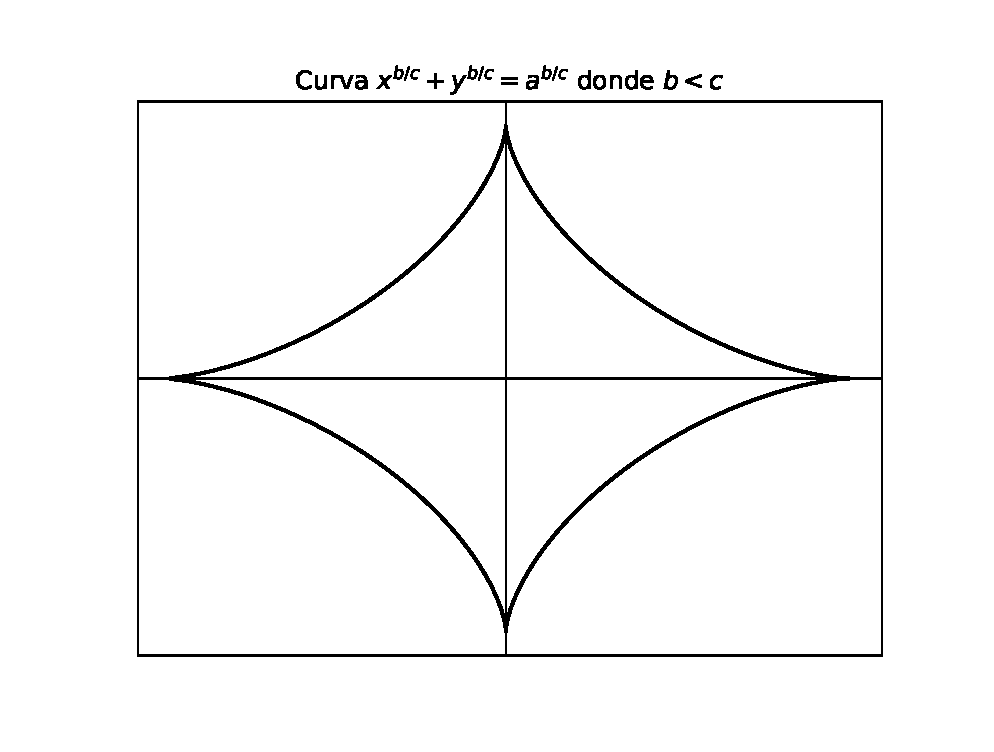
\includegraphics[scale=0.5]{Imagenes/plot_curva_estrella_01.eps}
    \caption{Estrella con cuatro picos cóncavos.}
    \label{fig:figura_curva_estrella}
\end{figure}
\end{frame}
\begin{frame}
\frametitle{Enunciado del problema}
Calcula el área dentro de la curva (ec. \ref{eq:ecuacion_curva_estrella}) en términos de la función Gamma cuando el exponente $b/c$ es $2/3$.
\end{frame}
\begin{frame}
\frametitle{Antes de la Solución}
Antes de resolver el problema, nos conviene observar que la familia de curvas representadas por la ecuación (\ref{eq:ecuacion_curva_estrella}) tiene como uno de sus miembros la conocida estrella de cuatro puntas o \emph{astroide}\footnote{También se le conoce como tetracúspide, cubocicloide, o paraciclo.}:
\begin{align*}
x^{2/3} + y^{2/3} = a^{2/3}
\end{align*}
\end{frame}
\begin{frame}
\frametitle{Antes de la Solución}
De hecho, siempre que $b < c$, se tiene una estrella cóncava con cuatro puntas afiladas (cúspides).
\\
\bigskip
Por otro lado, cuando $b > c$, la curva es convexa; y cuando $c = 1$ y $b$ es un entero par grande, la curva es casi un cuadrado.
\end{frame}
\begin{frame}
\frametitle{Antes de la Solución}
En cualquier caso, la curva es simétrica en ambos ejes de coordenadas, de modo que podemos \emph{calcular solo la parte del área que está en el primer cuadrante} y multiplicaremos el resultado por $4$ para obtener el área completa dentro de la curva.
\end{frame}
\begin{frame}
\frametitle{Antes de la solución}
\begin{figure}[H]
    \centering
    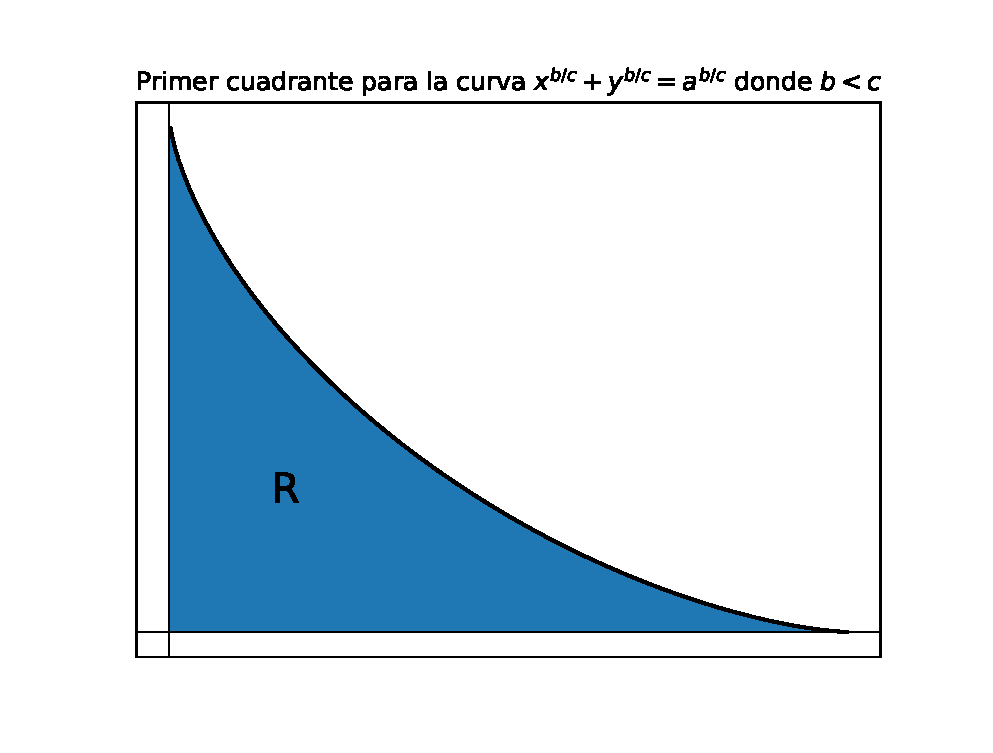
\includegraphics[scale=0.5]{Imagenes/plot_curva_estrella_02.eps}
    \caption{Cuadrante de trabajo para calcular el área.}
    \label{fig:figura_curva_estrella}
\end{figure}
\end{frame}
\begin{frame}
\frametitle{solución}
Obtendremos inicialmente una solución general para valores $a$, $b$ y $c$, posteriomente calcularemos la solución particular con los valores que nos da el enunciado: $b = 2$ y $c = 3$.
\end{frame}
\begin{frame}
\frametitle{Solución}
Tenemos entonces que:
\begin{align*}
\mbox{Área = } 4 \iint \limits_{R} \dd{A}
\end{align*}
donde $R$ representa la región en el primer cuadrante rodeado por la curva y los ejes.
\end{frame}
\begin{frame}
\frametitle{Solución}
Hacemos la doble integral a una integral equivalente con límites:
\begin{align*}
A = 4 \int_{0}^{a} \dd{x} \, \int_{0}^{\left( a^{b/c} - x^{b/c} \right)^{c/b}} \dd{y}
\end{align*}
\end{frame}
\begin{frame}
\frametitle{Cambio de variable para $y$}
Para evaluar la integral en $y$, hacemos el siguiente cambio de variable:
\begin{align*}
y = a \, v^{\frac{c}{b}} \hspace{1cm} \Longrightarrow \hspace{1cm} \dd{y} = a \, \left( \dfrac{c}{b} \right) \, v^{\frac{c}{b} - 1} \dd{v}
\end{align*}
\end{frame}
\begin{frame}
\frametitle{Cambio de variable para $x$}
Mientras estamos en eso, también podemos hacer el mismo tipo de cambio en la variable para $x$:
\begin{align*}
x = a \, u^{\frac{c}{b}} \hspace{1cm} \Longrightarrow \hspace{1cm} \dd{x} = a \, \left( \dfrac{c}{b} \right) \, u^{\frac{c}{b} - 1} \dd{u}
\end{align*}
\end{frame}
\begin{frame}
\frametitle{Nuevos límites de integración}
Al realizar los cambios de variables, corresponde entonces también realizar el cambio en los límites de integración, por lo tanto:
\begin{align*}
A = \dfrac{4 \, a^{2} \, c^{2}}{b^{2}} \, \int_{0}^{1} u^{\frac{c}{b} - 1} \dd{u} \, \int_{0}^{1-u} v^{\frac{c}{b} - 1} \dd{v}
\end{align*}
\end{frame}
\begin{frame}
\frametitle{Integrando con respecto a $v$}
Al realizar la integración con respecto a $v$, tenemos:
\begin{align*}
A = 4 \, a^{2} \, \left( \dfrac{c}{b} \right) \, \int_{0}^{1} u^{\frac{c}{b} - 1} (1 - u)^{c/b} \dd{u}
\end{align*}
\pause
Recordando que la función Beta se define como:
\begin{align*}
B(x, y) = \int_{0}^{1} t^{x-1} (1 - t)^{y-1} \dd{t} \hspace{1cm} x > 0, y > 0
\end{align*}
\end{frame}
\begin{frame}
\frametitle{Resultado parcial}
Encontramos una buena utilidad para las funciones que involucran integrales, ya que el cálculo de éstas se simplifica mucho.
\\
\bigskip
\pause
Entonces la integral anterior en la expresión para el área $A$, es la integral Beta, por tanto:
\end{frame}
\begin{frame}
\frametitle{Resultado parcial}
Tenemos que:
\begin{align*}
A = 4 \, \left( \dfrac{c}{b} \right) \, a^{2} \, B \left( \dfrac{c}{b}, \dfrac{c}{b} + 1 \right)
\end{align*}
\pause
Para resolver la expresión en términos mucho más sencillos, debemos de ocupar las propiedades e identidades para las funciones Gamma y Beta, como veremos a continuación:
\end{frame}
\begin{frame}
\frametitle{Ocupando propiedades}
Conocemos una expresión que relaciona la función Beta con la Gamma, entonces tendremos que:
\begin{align*}
A = 4 \, \left( \dfrac{c}{b} \right) \, a^{2} \, \left[ \dfrac{\mathlarger{\Gamma} \left( \dfrac{c}{b} \right) \, \mathlarger{\Gamma} \left( \dfrac{c}{b} + 1 \right)}{\mathlarger{\Gamma} \left( \dfrac{2 \, c}{b} + 1 \right)} \right]
\end{align*}
\end{frame}
\begin{frame}
\frametitle{Ocupando propiedades}
Seguimos ocupando las identidades de la función Gamma:
\begin{align*}
\mathlarger{\Gamma} \left( \dfrac{c}{b} + 1 \right) &= \dfrac{c}{b} \, \mathlarger{\Gamma} \left( \dfrac{c}{b} \right) \\[1em]
\mathlarger{\Gamma} \left( \dfrac{2 \, c}{b} + 1 \right) &= \dfrac{2 \, c}{b} \, \mathlarger{\Gamma} \left( \dfrac{2 \, c}{b} \right)
\end{align*}
\pause
Por lo que tenemos una expresión más sencilla que involucra la evaluación de la función Gamma, con los valores de $b$ y $c$, que nos devolverá una solución particular.
\end{frame}
\begin{frame}
\frametitle{Solución}
El área del astroide cuando $b = 2$ y $c = 3$ es:
\begin{align*}
A &= \dfrac{\mathlarger{\Gamma} \left( \dfrac{3}{2} \right) \, \mathlarger{\Gamma} \left( \dfrac{3}{2} \right)}{\mathlarger{\Gamma} (3)} \, (2) \left( \dfrac{3}{2} \right) \, a^{2} \\[1em]
&= \dfrac{3 \, a^{2} \, \pi}{8} \qed
\end{align*}
\end{frame}
\end{document}